\documentclass{article}
\usepackage{algpseudocode,extramarks,fancyhdr,paralist,amsmath,amsthm,amssymb,mathtools,url,graphicx,pdfpages,tikz,pdfpages,rotating,mathtools, hyperref, bm, hyperref,amsfonts,pgf,mathrsfs,xcolor,comment,mathdots,braket,physics}
\usepackage[plain]{algorithm}
\usepackage[utf8]{inputenc}

\usetikzlibrary{automata, positioning, decorations.pathmorphing, patterns, calc}

%
% Basic Document Settings
%

\topmargin=-0.45in
\evensidemargin=0in
\oddsidemargin=0in
\textwidth=6.5in
\textheight=9.0in
\headsep=0.25in

\linespread{1.1}

\pagestyle{fancy}
\lhead{\hmwkAuthorName}
\chead{\hmwkClass\ : \hmwkTitle}
\rhead{\firstxmark}
\lfoot{\lastxmark}
\cfoot{\thepage}

\newcommand{\dx}{\mathrm{d}x}
\newcommand{\solution}{\textbf{\large Solution}}
\newcommand{\E}{\mathrm{E}}
\newcommand{\Var}{\mathrm{Var}}
\newcommand{\Cov}{\mathrm{Cov}}
\newcommand{\Bias}{\mathrm{Bias}}
\newcommand{\lp}{\left(}
\newcommand{\rp}{\right)}
\newcommand{\bvec}{\vectorbold}
\newcommand{\di}{\mathrm{d}}
\setlength\parindent{0pt}
\newcommand{\uv}[1]{\hat{\bvec{#1}}}
\renewcommand{\grad}{\bvec{\nabla}}
\newcommand{\lap}{\bvec{\nabla}^2}
\renewcommand{\part}[2]{\partial_{#1}\left[ #2 \right]}
\newcommand{\bpart}[2]{\left[ #1 \right]_{#2}}
\newcommand{\bg}[1]{\begin{gather*} #1
\end{gather*}}

%
%Proof and theorem structure
%

\theoremstyle{definition} 
\newtheorem{theorem}{Theorem}
\newtheorem{lemma}[theorem]{Lemma}
\newtheorem{claim}[theorem]{Claim}
\newtheorem{corollary}[theorem]{Corollary}
\newtheorem{conjecture}[theorem]{Conjecture}
\newtheorem{definition}[theorem]{Definition}
\newtheorem{example}[theorem]{Example}
\newtheorem{remark}[theorem]{Remark}
\newtheorem{important}[theorem]{Important Note}
\newtheorem{recall}[theorem]{Recall}
\newtheorem{note}[theorem]{Note}
\newtheorem{question}[theorem]{Question}
\newtheorem*{definition*}{Definition}
\newtheorem*{theorem*}{Theorem}
\newtheorem*{claim*}{Claim}

%
%Prefreable integration method
%

\def\upint{\mathchoice%
    {\mkern13mu\overline{\vphantom{\intop}\mkern7mu}\mkern-20mu}%
    {\mkern7mu\overline{\vphantom{\intop}\mkern7mu}\mkern-14mu}%
    {\mkern7mu\overline{\vphantom{\intop}\mkern7mu}\mkern-14mu}%
    {\mkern7mu\overline{\vphantom{\intop}\mkern7mu}\mkern-14mu}%
  \int}
\def\lowint{\mkern3mu\underline{\vphantom{\intop}\mkern7mu}\mkern-10mu\int}

%
% Create Problem Sections
%

\newcommand{\enterProblemHeader}[1]{
    \nobreak\extramarks{}{Problem \arabic{#1} continued on next page\ldots}\nobreak{}
    \nobreak\extramarks{Problem \arabic{#1} (continued)}{Problem \arabic{#1} continued on next page\ldots}\nobreak{}
}

\newcommand{\exitProblemHeader}[1]{
    \nobreak\extramarks{Problem \arabic{#1} (continued)}{Problem \arabic{#1} continued on next page\ldots}\nobreak{}
    \stepcounter{#1}
    \nobreak\extramarks{Problem \arabic{#1}}{}\nobreak{}
}

\setcounter{secnumdepth}{0}
\newcounter{partCounter}
\newcounter{homeworkProblemCounter}
\setcounter{homeworkProblemCounter}{1}
\nobreak\extramarks{Problem \arabic{homeworkProblemCounter}}{}\nobreak{}

%
% Homework Problem Environment
%
% This environment takes an optional argument. When given, it will adjust the
% problem counter. This is useful for when the problems given for your
% assignment aren't sequential. See the last 3 problems of this template for an
% example.
%
\newenvironment{homeworkProblem}[1][-1]{
    \ifnum#1>0
        \setcounter{homeworkProblemCounter}{#1}
    \fi
    \section{Problem \arabic{homeworkProblemCounter}}
    \setcounter{partCounter}{1}
    \enterProblemHeader{homeworkProblemCounter}
}{
    \exitProblemHeader{homeworkProblemCounter}
}

%
% Homework Details
%   - Title
%   - Due date
%   - Class
%   - Section/Time
%   - Instructor
%   - Author
%
%----------------------------------------------------------------------------------------------------------------------------------------------------------------------------------
%----------------------------------------------------------------------------------------------------------------------------------------------------------------------------------
\newcommand{\hmwkTitle}{Homework\ \#4}
\newcommand{\hmwkDueDate}{Fri. Oct. 29th}
\newcommand{\hmwkClass}{Classical Mechanics 1}
\newcommand{\hmwkAuthorName}{\textbf{Harlan Heilman}}
%----------------------------------------------------------------------------------------------------------------------------------------------------------------------------------
%----------------------------------------------------------------------------------------------------------------------------------------------------------------------------------
%
% Title Page
%

\title{
    \vspace{2in}
    \textmd{\textbf{\hmwkClass\ }}\\
    \textmd{\textbf{\hmwkTitle\ }}\\
    \normalsize\vspace{0.1in}\small{Due\ on\ \hmwkDueDate\ }\\
    \vspace{3in}
}

\author{\hmwkAuthorName}
\date{}

%----------------------------------------------------------------------------------------------------------------------------------------------------------------------------------
%----------------------------------------------------------------------------------------------------------------------------------------------------------------------------------
%----------------------------------------------------------------------------------------------------------------------------------------------------------------------------------

\begin{document}

\maketitle

\pagebreak

\begin{homeworkProblem}
    Consider an equiliateral triangle of three equal masses $m$ and springs with spring constant $k$ and equilibrium length $l$ as discussed in class.  Consider this free to move in three dimensions (i.e. on the International Space Station).\\
    1.\ How many normal modes do you expect for this system?\\
    2.\ How many different frequencies do you expect?\\
    3.\ What would be the degeneracy of these frequencies?  Describe the modes with a sketch.\\
    4.\ Compute at least one non-zero frequency.\\
    \textbf{Solution}
    Lets start out with drawing the system 
    \begin{figure}[h]
        \centering
        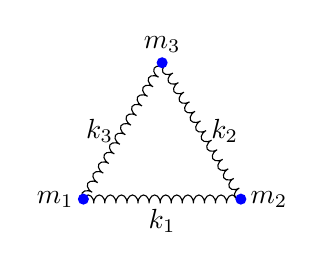
\begin{tikzpicture}
        \coordinate[label=left:{$m_1$}] (A) at (-1,0);
        \coordinate[label=above:{$m_3$}] (C) at (0, {sqrt(3)});
        \coordinate[label=right:{$m_2$}] (B) at (1,0);
        \coordinate[label=below:$k_1$] (D) at ($ (A)!.5!(B) $);
        \coordinate[label=right:$k_2$] (E) at ($ (B)!.5!(C) $);
        \coordinate[label=left:$k_3$] (F) at ($ (C)!.5!(A) $);        
        
        
        \draw[decoration={ segment length=4, amplitude=1.5, coil},decorate] (A) -- (B);
        \draw[decoration={ segment length=4, amplitude=1.5, coil},decorate] (A) -- (C);
        \draw[decoration={ segment length=4, amplitude=1.5, coil},decorate] (B) -- (C);
        
        \fill[blue] (A) circle [radius = 2pt];
        \fill[blue] (B) circle [radius = 2pt];
        \fill[blue] (C) circle [radius = 2pt];
        \end{tikzpicture}
    \end{figure}
    
    Now we will look at the various normal modes of this system. \\
    
    \textbf{Part 1.}\\
    Knowing that there are 3 masses, each with 2 degrees of freedom, there are going to be 6 total degrees of freedom in our system. This means that we could completely describe it with some position vector $\bvec{q} = (q_1\ q_2\ q_3\ q_4\ q_5\ q_6)^T$, and $\dot{\bvec{q}}$. Now when we move to normal modes, we hope to find behaviours of the system that more naturally describe its motion. Thus the system would more naturally be described by an eigenbasis of some operator, in this case, we will use the normal modes as the basis. But since these normal modes describe the same system, they must span a space of the dimension, so we will have 6 normal modes.\\
    
    In another sense, we will have a mode from translation of all of the masses along the $x$-axis, and a mode from translation of all the masses along the $y$-axis. This means translation corresponds to 2 modes. Now there must be 3 more modes that don't\\
    1)\ Cause a rotation about the center of mass\\
    2)\ Cause a translation of the center of mass\\
    If they did, then these normal modes would not be linearly dependent on the prior modes.\\
    
    The next group of normal modes come from oscillatory effects of each of the masses. The first of these is the breathing mode, all the masses move out from the center, or in towards the center. Now we need two more modes that come from the masses moving away from each other in a way that preserves the location of the center of mass and the causes no rotation. I will call these modes the pumping modes. 
    \\
    
    \textbf{Part 2.}
    Now we can look at the angular frequency corresponding to each of the. Since these are the eigenvalues corresponding to the normal modes of the system, there will be 6 angular frequencies. But, most of them will have some degeneracy.\\
    
    For example, right away, we know that the two transnational modes will have infinite period, and will thus have zero frequencies. Similarly, for small angles, as the triangle rotates, it's angle will be continuously increasing leading to a zero frequency.\\
    
    The remaining frequencies will be non zero.\\
    
    \textbf{Part 3.}
    As we said above, there are 3 normal modes that correspond with the eigenvalue $w^2 = 0$ (3 fold degeneracy). There are also frequencies that correspond to some amount of harmonic motion. Now, we will draw these out\\
    
    (See the drawn normal modes to the right. Tikz was being annoying and didn't want to compile)\\
    
    Lets start out with the breathing mode. Define $r$ as the distance from the center to the "node" $m_3$. But, since we define this mode as all the nodes move in or out the same amount, so $r(t)$ is the distance to any of the nodes at any time $t$. We will also define $d(t)$ as the length of the spring after each of the masses moves out or in, and $l$ is the equilibrium length of each spring. But, we can break one side of this triangle into two 30,60,90 triangles. This means we have the relationships 
    \[
        d = \sqrt{3}r,\ l = \sqrt{3}r_0
    \]
    Thus we can write the Lagrangian for this particular situation as 
    \[
        L = \frac{3m}{2}\dot{r}^2-\frac{9k}{2}(r+r_0)^2
    \]
    Since we are dealing with small oscillations, $r = r_0+\delta$, so the Lagrangian can be reduced to just depend on the small displacement $\delta$.
    \[
        L = \frac{3m}{2}\dot{\delta}^2-\frac{9k}{2}(\delta)^2
    \]
    Now we can do all the things that we do with Lagrangian Mechanics and get
    \[
        P_\delta = 3m\dot{\delta},\ \dot{P}_\delta = 3m\ddot{\delta} = -9k\delta
    \]
    But this means we have 
    \[
        m\ddot{\delta} = -3k\delta
    \]
    If we guess the form of $\delta = Ae^{i\omega t}$, we get
    \[
        m\omega^2Ae^{i\omega t} = 3kAe^{i\omega t}\iff \omega^2 = \frac{3k}{m}
    \]
    
    \par
    Note that if we take the normal mode described above and operate on it with any of the matrix representations of the symmetry group of an equilateral triangle, we get the same normal mode. So, this normal mode is a trivial representation of the $D_6$ group. 
    \\
    
    Now, lets think about changing the sign on one of the coordinates that rep presents the small displacement of one of the masses. If we are not careful here we will form a linearly dependent mode. So to fix this, we need to cancel out this change with a sign flip on another coordinate that small displacement for a second mass. These changes need to perfectly cancel each other out else we will have some transnational or rotational motion of the center of mass. This is exactly described by the drawings I made.\\
    
    If we now apply the symmetry operations to this displaced triangle, we find 3 different looking triangles, but we see that one of these can be formed with a linear combination of the other two. So these two linearly independent normal modes form a representation of the $D_6$ group. So, these normal modes will share the same angular frequency, and will have a twofold degeneracy. \\
    
    \textbf{Part 4}\\
    See part 3, but if we are careless with our notation and just set  $r = \delta$, the distance between the equilibrium position and the mass is nothing but 
    \[
        r(t) = r(0)e^{-\sqrt{3k/m}t}
    \]
\end{homeworkProblem}

\pagebreak

\begin{homeworkProblem}
    Repeat the process for a tetrahedron with four equal masses and four 6 equal springs. You may want to check your results with the code on CoCalc.\\
    
    \textbf{Solution}\\
    We know that there are now 3 degrees of freedom for each of the 4 masses. This means that we have 12 degrees of freedom and 12 normal modes for the system. We know that there will be translational modes in the x,y, and z axis. So this gives us 3 normal modes each with no angular frequency. Similarly, there are 3 normal modes corresponding to rotation about the x, y, and z axis, with no angular frequency for small angles. This means that there are 6 remaining normal modes that are caused by some form of oscillation.\\
    
    The remaining normal modes come from motion that cannot\\
    1)\ Cause traslation of the center of mass\\
    2)\ Cause rotation about the center of mass\\
    
    The next normal mode that we can call out is the breathing mode. All the masses get further away, or closer to the center of mass of the system. This means that the center of mass does not translate or rotate under this motion. Thus we have another normal mode, and we can clearly see that after a small displacement, there will be a restoring force and some angular frequency of the system, so the angular frequency will be non zero. This is the 1d representation of $D_{24}$\\
    
    Now we have to construct the 2d and 3d representations of $D_{24}$ from our normal modes. For the 2d representation, we will take inspiration from the stretching effect that happens in last two normal modes of the equilateral triangle. Lets start out with one of these squishing modes. If we add another mass and another dimension to the problem, we might guess that this mass will mirror one of the motions of the other 3 masses. So it has two options\\
    1)\ The mass must squish together and pull out with the other two masses that squish together\\
    2)\ The mass moves away from the center with the other mass that moves away from the center.\\
    
    Note that we might lose information by just taking the 2 linearly dependent modes, so to save ourselves, we will just take one and then apply the symmetry operations to determine the degeneracy of each angular frequency.\\
    
    Starting with the first option, we now need to choose one of the faces of the tetrahedron to squish in and pull pull out. There are 3 options for this, but just as in the 2d case, you can add all 3 modes together and get a zero displacement. So we now have a 2 fold degeneracy as opposed to a 3 fold one. 
    \\
    
    If we blindly apply the second option here, we see that each of these motions are some normal mode added to the breathing mode. This is because all the masses will move out form the center at the same rate, and two masses will move together and the other two masses will move apart. So if we throw out the breathing motion, we are left with a new normal mode of the system, two masses moving together, and two masses moving apart. But out of the 6 edges of the tetrahedron, we need to choose 2 to apply our motion rules to. But we cant have these edges touch, so we can throw out 9 of these modes. But since these motions are exactly $\pi$ out of phase with each other. So, when we rotate and reflect the tetrahedron such that the two masses that move together are in the same position as the masses that move apart, we have -1 times the same mode. This halves the motion back to just 3 normal modes, that are cyclic under the symmetry operations of the $D_{24}$ group. 
    \\
    
    Now lets find the angular frequency corresponding to the breathing mode of the tetrahedron. If we project everything into the plane, we have the same parameterization as the equilateral triangle, but we will call $r_p(t)$ (projected r) the distance between the center of the tetrahedron as projected into some plane that runs parallel to one of its surfaces. But from problem 1, $r_p = d\sqrt{3}$. So now we need to to find $r_p$ in terms of $r$. But, once more we have a 30,60,90 triangle. Thus we can write $r = 2r_p/\sqrt{3} = 2d/3$. We can do the same thing and find the equilibrium position of the masses. This means that the Lagrangian can be written as 
    \[
        L = 2m\dot{r}^2-2k(d-l)^2 = 2m\dot{r}^2-3k(r-r_0)^2
    \]
    But, $r = r_0+\delta$ where $\delta$ is a small displacement. Thus we can get out Lagrangian in terms of this small displacement as. 
    \[
        L = 2m\dot{\delta}^2-3k(\delta)^2
    \]
    So now we get 
    \[
        P_\delta = 4m\dot{\delta},\ \dot{P}_\delta = 4m\ddot{\delta} = -12k\delta
    \]
    If we guess the form of $\delta = Ae^{i\omega t}$, we get
    \[
        4m\omega^2Ae^{i\omega t} = 12kAe^{i\omega t}\iff \omega^2 = \frac{3k}{m}
    \]
    Now this is interesting. This equation leads to the same angular frequency as the normal mode of an equilateral triangle. But the systems have different total energies. This makes sense as there are three more springs that can store energy in their compression, and there is a fourth particle that can have kinetic energy. And, this is the same frequency in the third problem with equal masses and spring constants. So I would conject (but I don't have a solid proof) that all breathing normal modes with equal masses and spring constants have the same angular frequency. Anyways, we can write down the angular frequency that corresponds to the breathing mode as $\omega^2 = 3k/m$. 
    
\end{homeworkProblem}

\pagebreak

\begin{homeworkProblem}
    Provide a complete solution describing the motion of two coupled oscillators as shown
    below.\\
    
    Use your answer to characterize how energy is transferred between two harmonic
    oscillators.  I.e. consider the case where the middle spring has a very small spring
    constant $k_{12} \ll k_{1, 2}$.  This corresponds to two weakly coupled harmonic
    oscillators.  Suppose you excite the left oscillator with angular frequency $\omega_1
    \approx \sqrt{k_1/m_1}$: what conditions must be true in order that a significant
    portion of the energy can be transferred to the second oscillator with angular frequency
    $\omega_2 \approx \sqrt{k_2/m_2}$?
    \\
    
    \textbf{Solution}
    Since I am actively trying to build my intuition for this problem, I'm going to try to solve this backwards. If I where to plug this into a computer, I would start off with setting up two masses with 3 springs and give the system a kick. Then we could do a FFT and get the power spectrum of the system. Ideally i could do it a bunch of times and we would see two peaks for the two normal modes of the system. Then we could solve the problem and compare the angular frequencies to the normal modes. Now we could change the ratio of $k_{12}/k_{1,2}$ to see how the two masses are coupled together. \\
    
    My mind immediately jumps to quantum mechanics for this system. If we have a double square well, with a finite potential barrier between the two wells. If we put a particle in one of the wells, after some time the particle will tunnel though the barrier and appear in the other well. I would imagine that this is the behaviour that the energy of the system has. If we give one of the masses a kick, and leave the other at equilibrium, then the kinetic energy of the excited mass will transport to the stationary mass though the interactions with the springs. So why not throw this into a computer and have it give one of the particles a kick, and then plot the motion of the two particles. I imagine that the spring that couples the particles together will act somewhat like a damping force on one of the particles and a driving force on the other. But once "all" the kinetic energy has transferred to the second particle, we the coupling spring will damp the motion of the second particle and drive the motion of the 1st particle.\\
    
    Now the questions are, at what point does the coupling spring change from driving a mass to damping the mass? and What normal mode does this evolve into, and how long does it take for this evolution? Now I think that the system will devolve into one of the normal modes, and it will probably devolve into an anti symmetric mode (the masses moving in the same direction), but I don't have a great explanation as to why this is. The best explanation I have is looking at the out of sync metronomes set on a table. If you had two isolated metronomes where set far apart perhaps one on the ISS and the other in a lab on the earth, they would have no way of synchronising. But if you place them on the same table, after some time, the metronomes will synchronise their motion and move in an anti symmetric normal mode. As for the time it takes for the coupling spring to change from driving to damping, I would guess that it is dependent on $1/\omega_n$ where $\omega_n = \sqrt{k_2/m_2}$.\\
    
    Now, lets try to formulate the angular frequencies of the normal modes for this problem. Now, I want to force the asymptotic behavior for the symmetric normal mode that when $k = k_1 = k_{1,2} = k_2$, and $m = m_1 = m_2$, $\omega^2 = 3k/m$. Maybe the solutions will come as something like 
    \[
        \omega^2 = \frac{k_1\pm k_2\pm k_{12}}{\sqrt{m_1m_2}}
    \]
    The units work out here, and when we choose the right signs and follow the asymptotic behavior we want, we get breathing mode angular frequency, or the angular frequency of simple harmonic motion or one particle. Now if we let $k_{1,2}\to 0$, and have the masses and spring constants the same, we see that we either have
    \[
        \omega^2 = 0, \frac{2k}{m}
    \]
    and this makes sense as we have two decoupled harmonic oscillators. If their motion is out of phase, then the total system will have no angular frequency. But if they have the same angular frequency, then we have double the normal angular frequency.\\
    
    If we where to set up this system as an experiment, we could not totally decouple the experiment from the environment. So, we need to think about what we can decouple the system from. For example, if we set two independent simple harmonic oscillators with one spring and one mass on the same experimental table, they would couple though vibrations thought the table. So, we would need to properly separate the systems form the environment. Since the acceleration due to gravity is roughly constant at a lab scale, If it had any effect on the data, we could scale it out of our data. Similarly, the system does interact with the gravitational fields of all of the planets and stars in the universe, but these forces drop of with $1/r^2$, so its probably reasonable to throw out the effects of gravity on the system. We now also have to reduce the effect of friction and drag and whatnot, but these effects will just lead the system to relax to an equilibrium position (not exactly the equilibrium position of the spring, since the system will relax to the spot where the restoring forces cancel out the static friction forces). So there is some interesting physics when considering friction, but to me, the most important is thinking about the coupling of the two masses though the environment. \\
    
    Now lets actually find the normal modes of the problem. To do this, let $l$ be the equilibrium length of each spring. Then $\delta_i$ is the small displacement of the masses away from the equilibrium position. So, the kinetic energy is trivially, $K = \frac{1}{2}(m_1\dot{\delta_1}^2+m_2\dot{\delta_2}^2)$, but now we need to think about the equilibrium displacements of all the springs in the system. Lets first note that we could stretch the whole system, and apply a tension to all the springs in the system, but this will not do anything but add some global scale to the magnitude of all the forces in the system. So it's safe to say that the real equilibrium lengths of all the springs is $l$, and after some small displacement, the springs are now displaced by $d_1$,$d_2$, and $d_3$ respectively. Thus, the potential is nothing but $U = k_1(l-d_1)^2/2+k_{1,2}(l-d_2)^2/2+k_2(l-d_3)^2/2$. But, we need to determine $d_n$ in terms of the small displacement $\delta_i$. But, we can write these small displacements as 
    \begin{align*}
        d_1 & = l+\delta_1 & d_2 &= l-\delta_1+\delta_2 & d_3 & = l-\delta_2
    \end{align*}
    Thus the Lagrangian can be expressed in terms of the vector $\bvec{\delta} = (\delta_1 \ \delta_2)^T$, as 
    \[
        L = \frac{1}{2}(m_1\dot{\delta_1}^2+m_2\dot{\delta_2}^2) - \frac{1}{2}(k_1\delta_1^2+k_{1,2}\delta_1^2-2k_{1,2}\delta_1\delta_2+k_{1,2}\delta_{2}^2+k_2\delta_2^2)
    \]
    Since there are no cyclic variables, we cant jump into dealing with conserved quantities. So instead, we have the equations
    \begin{align*}
        \dot{P}_1 = m_1\ddot{\delta}_1 &= -k_1\delta_1+k_{1,2}(\delta_2-\delta_1)\\
        \dot{P}_2 = m_2\ddot{\delta}_2 &= -k_2\delta_2+k_{1,2}(\delta_1-\delta_2)
    \end{align*}
    Something we could have gotten by just using Newtons laws. But none the less, we want to find a orthonormal basis that describes the motion of the masses, so lets find the generalized eigenvectors (normal modes) of this matrix equation. So, we have the equation
    \[
    \begin{pmatrix}
    m_1 & o\\
    0 & m_2
    \end{pmatrix}
    \ddot{\vec{\delta}} = 
    -\begin{pmatrix}
    k_1+k_{1,2} & -k_{1,2}\\
    -k_{1,2} & k_2+k_{1,2}
    \end{pmatrix}
    \vec{\delta}
    \]
    But, when we guess that the equations come out as 
    \[
        \delta_i = A_ie^{i\omega t}
    \]
    We then reduce the equations following along with the general solution for these problems. Now lets just call $\delta_i = x_i$ for simplicity. 
    \[
        \begin{pmatrix}
        k_1+k_{1,2}-m_1\omega^2 & -k_{1,2}\\
        -k_{1,2} & k_2+k_{1,2}-m_2\omega^2
        \end{pmatrix}
        \vec{X} = \vec{0}
    \]
    We only have non trivial solutions when the determinant on the left is equal to zero. Thus we have the characteristic equation, 
    \[
        (k_1+k_{1,2}-m_1\omega^2)(k_2+k_{1,2}-m_2\omega^2) - k_{1,2}^2 = 0
    \]
    \[
        k_1k_2+k_1k_{1,2}+k_2k_{1,2}-m_2\omega^2k_1-m_1\omega^2k_{1,2}-m_1\omega^2k_2 - m_2\omega^2k_{1,2} + m_1m_2\omega^4= 0
    \]
    To make my life easier, lets do the following 
    \begin{align*}
        k_1k_2+k_1k_{1,2}+k_2k_{12} &= \kappa\\
        m_2k_{1,2}+m_1k_2+m_1k_{1,2}+m_2k_1 &= \gamma' = M^2(k_{1,2}/m_1+k_2/m_2+k_{1,2}/m_2+k_1/m_1) = M^2\gamma\\
        m_1m_2 &= M^2
    \end{align*}
    So now, we have the quadratic equation. 
    \[
        \kappa-\gamma\omega^2+M^2\omega^4 = 0
    \]
    Solving this with the quadratic equation, we get 
    \[
        \omega^2 = \frac{\gamma'\pm\sqrt{\gamma'^2-4M^2\kappa}}{2M^2} = \frac{\gamma}{2}\pm\frac{\sqrt{\gamma^2-4(\kappa/M^2)}}{2}
    \]
    Now I am sure that we can simplify this further bu inputting the substitutions that where suggested, but now I see that what I have here reduces to exactly what I want when the masses and spring constants are the same. And I can mess around with a small $k_{1,2}$ rather readily. There is one last substitution that I will make to make my life easier. That is, let
    \[
        \beta = \left(\frac{k_{1,2}^2}{m_2^2}+\frac{k_{1,2}^2}{m_1^2}+\frac{k_1^2}{m_2^2}+\frac{k_2^2}{m_1^2}+\frac{2k_{1,2}^2}{m_1m_2}+\frac{2k_{1,2}k_1}{m_1^2}+\frac{2k_{1,2}k_2}{m_2^2}-\frac{2k_1k_2}{m_1m_2}-\frac{2k_1k_{1,2}}{m_1m_2}-\frac{2k_2k_{1,2}}{m_1m_2}\right) = \gamma^2-4(\kappa/M^2)
    \]
    Now the equations for the angular frequencies are 
    \[
        \omega^2 = \frac{\gamma}{2}\pm\frac{\sqrt{\beta}}{2}
    \]
    Lets verify that this reduces to what we want when $k_1 = k_2 = k_{1,2}$, and $m_1 = m_2$. We see that $\beta = 4k^2/m^2$, $\gamma = 4k/m$. So we have $\omega^2 = 2k/m\pm k/m$, and we get the angular frequencies that we want. This equation is still too messy to give me anything useful when it comes to finding the normal modes, and I'm not sure how to simplify it more. I can get rid of the fractions by replacing my masses and spring constants with frequencies. This would be fine, except now it is borderline impossible to find the exact form of the normal modes without going crazy from algebra. So, I will go ahead and make the simplification that the spring constants $m_1 = m_2 = m$, and $k_1 = k_2$. Then after taking the determinant, I have 
    \[
        (k+k_{1,2}-m\omega^2)^2-k_{1,2}^2 = 0 \iff \omega^2 = \frac{k}{m},\ \frac{k+2k_{1,2}}{m}
    \]
    so now, plugging these values back into the matrix equation gives,
    \[
        k_{1,2}\begin{pmatrix}
        1 & -1\\
        -1 & 1
        \end{pmatrix} \vec{X} = \vec{0} \iff \vec{X} = \begin{pmatrix}
        1\\
        1
        \end{pmatrix}
    \]
    and 
    \[
        -k_{1,2}\begin{pmatrix}
        1 & 1\\
        1 & 1
        \end{pmatrix} \vec{X} = \vec{0} \iff \vec{X} = \begin{pmatrix}
        1\\
        -1
        \end{pmatrix}
    \]
    Thus we can write out the equations for each of the normal modes as 
    \begin{align*}
        \delta_1(t) = A_1e^{i\omega_1t}+A_2e^{i\omega_1t}\\
        \delta_2(t) = A_1e^{i\omega_2t}-A_2e^{i\omega_2t}
    \end{align*}
    
    Lets now move to analysing the transfer of energy between the two masses. If we let one mass start off initially with some displacement $A$, and no initial velocity, and we force the other mass to be held at its equilibrium position, we can analyse this. But since we have one mass starting with an initial displacement, and the other starting with no displacement, we can jump to the solutions to a simple harmonic oscillator. 
    \[
        \delta_1 = A(\cos(w_1t)+\cos(w_2t))/2,\ \delta_2 = A(\cos(w_1t)-\cos(w_1t))/2
    \]
    But calling back to the cheating I did, $\omega_0^2 = k/m$, and $\omega_1^2 = \frac{k+2k_{1,2}}{m}$. So as $k_{1,2}<<k$, the difference between these frequencies gets smaller and smaller (This seams like we are building up to something like beats but applied to discrete masses). So, now if we take their average frequency, 
    \[
        \omega_0 = \frac{\omega_2+\omega_1}{2}
    \]
    then we can say that each of $\omega_1$ and $\omega_2$ are $\epsilon$ away from the average frequency, for $\epsilon$ small. Thus we have 
    \[
        \delta_1 = A(\cos(w_0-\epsilon)t+\cos(w_0+\epsilon)t)/2,\ \delta_2 = A(\cos(w_0-\epsilon)t-\cos(w_0+\epsilon)t)/2
    \]
    But this reduces to 
    \[
        \delta_1 = A\cos(\omega_0t)\cos(\epsilon t),\ \delta_2 = A\sin(\omega_0t)\sin(\epsilon t)
    \]
    So, we see that my initial prediction was correct, and slowly the left side mass decreases it's amplitude and the right side mass begins motion. I think my explanation of one mass driving the other works out. But, my initial formula from the start does not work. I had a theory that the the time it would take for a one particle to go from driving to damping the other would be dependent on the frequency difference between the two oscillators, but i never tried to express it. But now, we see that explicitly in the equations. Where $2\epsilon$ is the difference between the frequency of each of the particles. I also feel like my initial assumption that these masses are exactly like metronomes on a table is incorrect, since without energy loss to the environment, the masses will never reach a point where their phase difference goes to zero.\\
    
    But, I now need to get a good answer for what conditions must be met for a significant portion of the energy to be transferred to the second oscillator. I think that as long as the oscillators are coupled. Now if we want to distinguish between energy being transferred from mass 1 to mass 2, then we would want to say that while $t<\pi/2\epsilon$ the kinetic energy of mass 1 is being transferred though the springs into kinetic energy for mass 2. From that point onward, until $t = \pi/\epsilon$, the second mass slowly looses energy as it drives the motion of the first mass.
    \\
    
    Now my next step would be to plug this into a computer and figure out what I was careless about in my analysis. But, I ran out of time, so Ill try it out this weekend and see what comes of it. I know that the dimensions of my equations come out correct since when I checked the limiting cases, I returned to the results for 2 equal masses and 3 equal springs. I can't think of other coordinate systems that we could look at that would give us any good information about the system. The center of mass coordinates would give us no information for symmetric oscillations. We could pick an accelerating frame from the surface of one of the boxes, but that seams not very useful to me. I need to sit with this problem some more and force the algebra to give me something useful, because right now I cant see thought the general solution and compare it to my predicted general solution. 
    
\end{homeworkProblem}

\end{document}
%----------------------------------------------------------------------------------------------------------------------------------------------------------------------------------
%----------------------------------------------------------------------------------------------------------------------------------------------------------------------------------
%----------------------------------------------------------------------------------------------------------------------------------------------------------------------------------
